%!TEX root = ../thesis.tex
%*******************************************************************************
%****************************** Second Chapter *********************************
%*******************************************************************************

\chapter{Case Study}

\ifpdf
    \graphicspath{{Chapter2/Figs/Raster/}{Chapter2/Figs/PDF/}{Chapter2/Figs/}}
\else
    \graphicspath{{Chapter2/Figs/Vector/}{Chapter2/Figs/}}
\fi


\section{Introduction to the project}

In this paper, I present the design, implementation, and preliminary testing of an AI–powered conversational assistant (CA) prototype, whose scope is to assist psychiatric nurses in their day-to-day treatments. The assistant built is nurse-facing (not patient-facing), and its role is to assist nurses in performing the concrete task of accessing on the spot and in natural language important pieces of information about a patient's profile (e.g. medications prescribed, etc.). This assistant is designed to interact with users, comprehend their queries, and provide on-demand, insightful information sourced from a medical database.

For this prototype, hypothetical data were used, and protected health information (PHI) was not included.

This work aims at answering the following research questions \label{RQs}:
\begin{itemize}
    \item RQ1) Is it feasible to develop a CA that helps nurses to extract information about a patients' profiles on demand?
    \item RQ2) If so, how effective is the CA in terms of faithfulness, answer relevancy and answer correctness, context precision and context recall ?
    \item RQ3) Is it effective? Does the CA improve the daily experience and satisfaction for the job of the nurse?
\end{itemize}

\section{Requirements Gathering and Design}
Usually, the design and development of dialog systems begins with the collection and analysis of sample dialogs between real people (e.g. between health providers and patients) \cite{BickmoreGiorgino2006}. The recordings are then transcribed and analyzed carefully to understand the range of topics, concepts, terms, and general structure typically used in patient–physician communication. However, for the particular project -- as well as for most industry-led ones -- there were no real template-dialogs to be followed, due to GDPR regulations, and the ethical principle of medical confidentiality, both of which prohibit the dissemination of medical conversations and data. The requirements gathering phase was implemented through interviews with professional psychiatric nurses.

The design process, from project start to completion of the user studies, lasted three months (November 2024 to January 2025). During this period, I interviewed three nurses who worked in psychiatric clinics. Their experience and insights helped me learn about the stakeholders and the basic workflow requirements of the system.

Three psychiatric nurses were interviewed for 2 hours each, over Zoom during the month of November, 2024. The interviewed nurses gave information voluntarily about what psychiatric care in Greek psychiatric clinics involves. They explained the different psychiatric facilities, the daily tasks of a nurse during a typical shift, what a nurse should pay attention to when dealing with patients, and how they collaborate with the rest of the medical team, i.e. doctors, psychologists, and social workers. From the discussions, certain ``pain points`` emerged. 

First, the daily job of a psychiatric nurse is critical and very demanding, since nurses are responsible for the following tasks:
\begin{enumerate}
    \item observe the patients at all times, so they do not harm themselves or others
    \item make sure the patients do not flee the clinic
    \item get to know the patients well, mainly in order to understand who can pose a threat to themselves or others
    \item administer medication and make sure the patients actually swallow it
    \item convince the patients to follow their medication treatment, and set goals about their health 
    \item monitor the patients and change their medication or their doses
    \item liaise with other medical specialists (e.g. cardiologist, ophthalmologist, etc.) on behalf of the patients, and accompany them during visits
\end{enumerate}
Notably, there is no specific patient assigned to each nurse; rather, all nurses are responsible for all patients, and any nurse can observe and treat any patient.

Second, there are no comprehensive electronic patient records.  A full record for each patient exists as hand-written notes from the relevant medical professionals, called ``Patient Record``, and includes information on the patient's demographic status (sex, age, etc.), social life (if they have a family, a social network, a job, etc.), medical history (their symptoms and diagnosis, hospitalization dates, other medical conditions, etc.), and psychological profile (their desires, dislikes, fears, etc.). Interestingly, there exists only one record for each patient (without extra copies), and it is updated manually in the event of a patient's readmission. There are, however, a few pieces of information that can also be retrieved electronically via the patient's Social Security Number (AMKA), that is the patient's medication regimen (i.e. dosage, schedule, duration pf treatment), the doctor who prescribed it, and their admission and discharge dates. 

All three nurses expressed their excitement for a phone application that would aid them in their job. As a suggestion, they offered the following: having an assistant that knows pieces of information about each patient, which are personal to each nurse and customized by her/him. This customized patient record would help nurses in accessing important data about a specific patient on the spot, without the need to refer to the unique copy of the official, hand-written Patient Record, or rely on memory. 

The resulting requirements and expectations were the following:
\begin{enumerate}
\item The assistant will not take the initiative to speak, but will answer questions asked by the nurse fast and reliably, in both voice and text format
\item Voice-enabled for fast note recording and for hearing brief pieces of information on demand (e.g. - ``Who prescribed medication A? ``, -  ``Doctor X``)
\item Text-enabled for reading longer notes (e.g. a summary of the medical history) and committing to memory
\item Data that would be helpful are:
\begin{itemize}
    \item Medical Record Number (AMKA)
    \item Cellphone of patient or of a contact
    \item Diagnosis (name and date)
    \item Admission and discharge dates, if any
    \item Prescribed treatment plan (doses and schedule)
    \item Past side-effects of drugs
    \item Last injection and next injection
    \item Past blood tests and next blood tests
    \item Evaluation of patient's adherence to the medical plan
    \item Evaluation of patient's mental and physical health
    \item Brief social profile
    \item Important advice or warning from the doctor
\end{itemize}       
Symptoms are well-known to the nurses, so they are not included in the data.
\end{enumerate}

\subsection{Objective}
The objective of the AI assistant was to reduce the time and effort needed to retrieve relevant and accurate information about patients. This would also streamline their workflow, increase the speed and accuracy of the nurses' decisions for each patient, and would ultimately improve their quality of healthcare.

\section{Scenarios of multi-turn interactions in Greek}
\subsection{Happy Paths}
\subsubsection{Scenario 1: Memory}
\begin{table}[H]
\centering
\renewcommand{\arraystretch}{1.5} 
\begin{tabular}{|>{\bfseries}l|p{11cm}|}
\hline
Nurse & \textgreek{Η Μαρία Παπαδοπούλου τι αγωγή παίρνει στην παρούσα φάση?} \\
\hline
System - golden & \textgreek{Η Μαρία Παπαδοπούλου παίρνει αλπραζολάμη για τις κρίσεις πανικού με δοσολογία 0,5 mg και πρόγραμμα 2 φορές την ημέρα.} \\
\hline
System - actual & \textgreek{Η Μαρία Παπαδοπούλου λαμβάνει αλπραζολάμη (0.5 m}g) \textgreek{2 φορές την ημέρα για τις κρίσεις πανικού, σύμφωνα με συνταγή του ιατρού Γιάννη Γαστουνιώτη.} \\
\hline
Nurse & \textgreek{Και σε ποια ουσία έχει παρενέργειες?} \\
\hline
System - golden & \textgreek{Στο λίθιο.} \\
\hline
System - actual & \textgreek{Στα έγγραφα της Μαρίας Παπαδοπούλου αναφέρονται παρενέργειες για το λίθιο, το οποίο η ίδια διέκοψε την 1η Οκτωβρίου 2023. Οι παρενέργειες του λιθίου είναι αυξημένη ορμόνη} TSH  \textgreek{(υποθυρεοειδισμός), καταστολή και υπνηλία και τρέμουλο στα χέρια. Δεν αναφέρονται παρενέργειες για την αλπραζολάμη.} \\
\hline
\end{tabular}
\caption{Scenario 1 (audios 1, 2): Memory - MARIA}
\end{table}

\subsubsection{Scenario 2: Memory and reference resolution}
\begin{table}[H]
\centering
\renewcommand{\arraystretch}{1.5} 
\begin{tabular}{|>{\bfseries}l|p{11cm}|}
\hline
Nurse & \textgreek{Πότε έγιναν οι προηγούμενες αιματολογικές εξετάσεις του Κώστα Καρά?} \\
\hline
System - golden & \textgreek{Στις 24/11/2024.} \\
\hline
System - actual & \textgreek{Οι προηγούμενες αιματολογικές εξετάσεις του Κώστα Καρά έγιναν στις 10/02/2024 και 24/11/2024.} \\
\hline
Nurse & \textgreek{Και οι επόμενες εξετάσεις του?} \\
\hline
System - golden & \textgreek{Στις 15/5/2025.} \\
\hline
System - actual & \textgreek{Οι επόμενες αιματολογικές εξετάσεις του Κώστα Καρά είναι προγραμματισμένες για τις 15/5/2025.} \\
\hline
Nurse & \textgreek{Τι συστάσεις υπάρχουν?} \\
\hline
System - golden & \textgreek{Προώθηση ψυχοθεραπείας για διαχείριση άγχους και καθοδήγηση για ενίσχυση κοινωνικών δεξιοτήτων.} \\
\hline
System - actual & \textgreek{Οι τρέχουσες ιατρικές συστάσεις για τον Κώστα Καρά περιλαμβάνουν την προώθηση ψυχοθεραπείας για διαχείριση άγχους και καθοδήγηση για ενίσχυση κοινωνικών δεξιοτήτων.} \\
\hline
\end{tabular}
\caption{Scenario 2 (audios 3, 4, 5): Memory and reference resolution - KOSTAS}
\end{table}

\subsubsection{Scenario 3: Abbreviations and Acronyms}
\begin{table}[H]
\centering
\renewcommand{\arraystretch}{1.5} 
\begin{tabular}{|>{\bfseries}l|p{11cm}|}
\hline
Nurse & \textgreek{Η Δήμητρα Τσακίρη τι διάγνωση έχει?} \\
\hline
System - golden & \textgreek{ΓΑΔ (διάγνωση το 16/04/2004) και κρίσεις πανικού (διάγνωση το 23/01/2008)} \\
\hline 
System - actual & \textgreek{Η Δήμητρα Τσακίρη έχει διαγνωστεί με ΓΑΔ (Γενικευμένη Αγχώδης Διαταραχή) στις 16/04/2004 και με κρίσεις πανικού στις 23/01/2008.} \\
\hline
Nurse & \textgreek{Πες μου τη δοσολογία της αγωγής για την Ιωάννα Λυμπερίου.} \\
\hline
System - golden & \textgreek{Δραστική ουσία: κουετιαπίνη
Δοσολογία: 300} mg, \textgreek{2 φ/ημ.} \\
\hline
System - actual & \textgreek{Η Ιωάννα Λυμπερίου λαμβάνει κουετιαπίνη σε δοσολογία 300} mg, \textgreek{2 φορές την ημέρα. Η έναρξη της αγωγής ήταν στις 30/08/2018 και συνταγογραφήθηκε από τον καρδιολόγο Ιωάννη Μακρή.} \\
\hline
Nurse & \textgreek{Δώσε μου το τηλέφωνο και το ΑΜΚΑ του Γιώργου Γεωργίου.} \\
\hline
System - golden & \textgreek{Τηλ.: 6974513248 (μητέρα, κα. Αθανασία) και ΑΜΚΑ: 67980831881} \\
\hline
System - actual & \textgreek{Το ΑΜΚΑ του Γιώργου Γεωργίου είναι 67980831881 και το τηλέφωνο είναι 6974513248 (της μητέρας του, κα. Αθανασίας).} \\
\hline
Nurse & \textgreek{Γιώργος Μακρής. Τι διαγνώσεις έχει?} \\
\hline
System - golden & \textgreek{- Κρίσεις πανικού (διάγνωση το 12/11/2002)
- Διπολική διατ. (διάγνωση το 15/01/2021)
- Ψύχωση (διάγνωση το 25/04/2012)} \\
\hline
System - actual & \textgreek{Ο Γιώργος Μακρής έχει διαγνωστεί με τα εξής: Κρίσεις πανικού (12/11/2002), Διπολική διαταραχή (15/01/2021) και Ψύχωση (25/04/2012).} \\
\hline
\end{tabular}
\caption{Scenario 3 (audios 6, 7, 8, 9): Abbreviations and Acronyms - PATIENT 01 and PATIENT 03 and PATIENT 04 and PATIENT 05}
\end{table}

 
\subsection{Error Scenarios}
\subsubsection{Scenario 4: Non-existent patient}
\begin{table}[H]
\centering
\renewcommand{\arraystretch}{1.5} 
\begin{tabular}{|>{\bfseries}l|p{11cm}|}
\hline
Nurse & \textgreek{Σε ποια ουσία έχει παρενέργειες η Δήμητρα Καρακίτσου?} \\
\hline
System - golden & \textgreek{Δεν ξέρω.} \\
\hline
System - actual & \textgreek{Δεν βρέθηκαν πληροφορίες σχετικά με το σε ποια ουσία έχει παρενέργειες η Δήμητρα Καρακίτσου.} \\
\hline
\end{tabular}
\caption{Scenario 4 (audio 10): Non-existent patient}
\end{table}

\subsubsection{Scenario 5: Non-existent patient who shares the same last name with a known patient}
\begin{table}[H]
\centering
\renewcommand{\arraystretch}{1.5} 
\begin{tabular}{|>{\bfseries}l|p{11cm}|}
\hline
Nurse & \textgreek{Πες μου τις συστάσεις για την ασθενή Θάλεια Παπαδοπούλου.} \\
\hline
System - golden & \textgreek{Δεν ξέρω.} \\
\hline
System - actual & \textgreek{Δεν βρέθηκαν πληροφορίες για την ασθενή Θάλεια Παπαδοπούλου.} \\
\hline
\end{tabular}
\caption{Scenario 5 (audio 11): Non-existent patient who shares the same last name with a known patient}
\end{table}

\subsubsection{Scenario 6: Known patient with non-existent info}
\begin{table}[H]
\centering
\renewcommand{\arraystretch}{1.5} 
\begin{tabular}{|>{\bfseries}l|p{11cm}|}
\hline
Nurse & \textgreek{Πότε είναι η επόμενη ενέσιμη αγωγή του Κώστα Καρά?} \\
\hline
System - golden & \textgreek{Δεν έχει ενέσιμη αγωγή.} \\
\hline
System - actual & \textgreek{Ο Κώστας Καράς δεν έχει ενέσιμη αγωγή. Έχει όμως προγραμματισμένες αιματολογικές εξετάσεις στις 15/5/2025.} \\
\hline
\end{tabular}
\caption{Scenario 6 (audio 12): Known patient with non-existent info - KOSTAS}
\end{table}

\subsubsection{Scenario 7: Doctor's name}
\begin{table}[H]
\centering
\renewcommand{\arraystretch}{1.5} 
\begin{tabular}{|>{\bfseries}l|p{11cm}|}
\hline
Nurse & \textgreek{Πες μου το ΑΜΚΑ της Κωνσταντίνας Λυμπερίου.} \\
\hline
System - golden & \textgreek{Δεν ξέρω.} \\
\hline
System - actual & \textgreek{Δεν βρέθηκαν δεδομένα για την Κωνσταντίνα Λυμπερίου. Δεν μπορώ να σου δώσω το ΑΜΚΑ της.} \\
\hline
\end{tabular}
\caption{Scenario 7 (audio 13): Doctor's name - GEORGIA M}
\end{table}

\subsection{Disambiguation Scenarios}
\subsubsection{Scenario 8: Disambiguation of identical patient name}
\begin{table}[H]
\centering
\renewcommand{\arraystretch}{1.5} 
\begin{tabular}{|>{\bfseries}l|p{11cm}|}
\hline
Nurse & \textgreek{Θύμισέ μου το κοινωνικό ιστορικό της Ελένης Κανελλοπούλου.} \\
\hline
System & \textgreek{Έχω βρει πληροφορίες για δύο ασθενείς με το όνομα Ελένη Κανελλοπούλου. Η μία είναι 54 ετών (ΑΜΚΑ: 63681990357) και η άλλη είναι 41 ετών (ΑΜΚΑ: 65357602736). Για ποια από τις δύο Ελένες Κανελλοπούλου θέλετε το κοινωνικό ιστορικό?} \\
\hline
Nurse & \textgreek{Πες μου για τη μεγαλύτερη.} \\
\hline
System - golden & PATIENT 15.txt \\
\hline
System - actual & \textgreek{OK. Το κοινωνικό ιστορικό της Ελένης Κανελλοπούλου (ΑΜΚΑ: 63681990357) είναι:
*   Μένει μόνη σε ενοικιαζόμενο διαμέρισμα
*   Έχει ελάχιστη οικογενειακή υποστήριξη
*   Δεν εργάζεται επί του παρόντος
*   Πρώην υπάλληλος γραφείου, αποχώρησε λόγω επιδείνωσης της ψυχικής υγείας
*   Διατηρεί περιορισμένη επαφή με μία εξαδέλφη. Όσον αφορά τις συνήθειες και την καθημερινότητά της:
*   Καπνίζει περίπου 10 τσιγάρα την ημέρα
*   Δεν καταναλώνει αλκοόλ
*   Παρουσιάζει διαταραχές ύπνου (δυσκολία έναρξης και διατήρησης ύπνου, συχνές διακοπές για ούρηση)
*   Βλέπει τηλεόραση και ράβει για να ηρεμεί.
Οι συστάσεις για την Ελένη Κανελλοπούλου είναι:
*   Συστηματική ψυχοθεραπεία και παρακολούθηση
*   Ενίσχυση κοινωνικών δεξιοτήτων μέσω ομάδων υποστήριξης
*   Εκπαίδευση στη διαχείριση στρες και τεχνικές αναπνοής
*   Συμμετοχή σε πρόγραμμα επανένταξης στην εργασία (ΔΥΠΑ)
*   Προγραμματισμός αξιολόγησης από Κοινωνική Υπηρεσία για πιθανή παροχή βοήθειας κατ’ οίκον.} \\
\hline
\end{tabular}
\caption{Scenario 8 (audio 14, 15): Disambiguation of identical patient name - PATIENT 13 and PATIENT 15}
\end{table}

\subsubsection{Scenario 9: Disambiguation of identical patient name and double intent}
\begin{table}[H]
\centering
\renewcommand{\arraystretch}{1.5} 
\begin{tabular}{|>{\bfseries}l|p{11cm}|}
\hline
Nurse & \textgreek{Πότε νοσηλεύτηκε τελευταία φορά η Δήμητρα Μακρή και τι αγωγή παίρνει?} \\
\hline
System & \textgreek{Υπάρχουν δύο ασθενείς με το όνομα Δήμητρα Μακρή. Για να σας δώσω τις σωστές πληροφορίες, θα μπορούσατε να επιβεβαιώσετε τον ΑΜΚΑ ή την ηλικία της ασθενούς για την οποία ενδιαφέρεστε?} \\
\hline
Nurse & \textgreek{Δε θυμάμαι το ΑΜΚΑ της. Πες μου για την πιο μικρή.} \\
\hline
System - golden &  \textgreek{Στις 20/03/2013: Επιθετικό-μανιακό πεισόδιο με παραμονή 2 ημέρες, και στις 27/09/2017: Επεισόδιο σχιζοφρένειας με παραμονή 1 ημέρες. Παίρνει ρισπεριδόνη, 3 mg, 2 φορές την ημέρα, και ζιπραζιδόνη, 40 mg, 2 φορές την ημέρα μαζί με φαγητό.} \\
\hline
System - actual & \textgreek{Η Δήμητρα Μακρή, 32 ετών (ΑΜΚΑ 41661927592), νοσηλεύτηκε τελευταία φορά στις 27/09/2017 και λαμβάνει ρισπεριδόνη (3 mg, 2 φ. την ημέρα) και ζιπραζιδόνη (40 mg, 2 φ. την ημέρα μαζί με φαγητό).} \\
\hline
\end{tabular}
\caption{Scenario 9 (audio 16, 17): Disambiguation of identical patient name and double intent - PATIENT 10 and PATIENT 16}
\end{table}

\subsubsection{Scenario 10: Free-form text}
\begin{table}[H]
\centering
\renewcommand{\arraystretch}{1.5} 
\begin{tabular}{|>{\bfseries}l|p{11cm}|}
\hline
Nurse & \textgreek{Θύμισέ μου αν ακολουθεί τη θεραπεία της η Βασιλική Αντωνίου.} \\
\hline
System - golden & \textgreek{Λαμβάνει τα φάρμακά της με σχετική συνέπεια, αν και παρατηρούνται περιστασιακές παραλείψεις, κυρίως κατά τις περιόδους ύφεσης. 
Παρουσιάζει μειωμένη αυτογνωσία σχετικά με την ανάγκη για συνεχή θεραπεία, γεγονός που αποδίδεται εν μέρει σε μερική ανοσογνωσία.} \\
\hline
System - actual & \textgreek{Η Βασιλική Αντωνίου λαμβάνει τα φάρμακά της με σχετική συνέπεια, αν και παρατηρούνται περιστασιακές παραλείψεις, κυρίως κατά τις περιόδους ύφεσης. Παρουσιάζει μειωμένη αυτογνωσία σχετικά με την ανάγκη για συνεχή θεραπεία, γεγονός που αποδίδεται εν μέρει σε μερική ανοσογνωσία.} \\
\hline
Nurse & \textgreek{Έχει κάποιες συστάσεις στο φάκελό της?} \\
\hline
System - golden & \textgreek{Οι θεραπευτικές κατευθύνσεις περιλαμβάνουν τη συνέχιση της φαρμακευτικής αγωγής υπό τακτική παρακολούθηση, την επανένταξή της σε ομάδα υποστηρικτικής ψυχοθεραπείας σε εβδομαδιαία βάση, την καθιέρωση ενός σταθερού προγράμματος δραστηριοτήτων που να περιλαμβάνει βόλτες και ελαφριές οικιακές εργασίες, καθώς και τη συμμετοχή σε πρόγραμμα κοινωνικοποίησης στο κέντρο ημέρας. 
Επιπλέον, προτείνεται παραπομπή σε ψυχολόγο για γνωσιακή-συμπεριφορική θεραπεία, παροχή συμβουλευτικής υποστήριξης προς την οικογένειά της, ενίσχυση της αίσθησης αυτοαποτελεσματικότητας και ενδυνάμωσης, και μηνιαία παρακολούθηση από κοινωνικό λειτουργό.} \\
\hline
System - actual & \textgreek{Ναι, υπάρχουν κάποιες συστάσεις στο φάκελο της Βασιλικής Αντωνίου. Προτείνεται παραπομπή σε ψυχολόγο για γνωσιακή-συμπεριφορική θεραπεία, παροχή συμβουλευτικής υποστήριξης προς την οικογένειά της, ενίσχυση της αίσθησης αυτοαποτελεσματικότητας και ενδυνάμωσης, και μηνιαία παρακολούθηση από κοινωνικό λειτουργό. Επιπλέον, οι θεραπευτικές κατευθύνσεις περιλαμβάνουν τη συνέχιση της φαρμακευτικής αγωγής υπό τακτική παρακολούθηση, την επανένταξή της σε ομάδα υποστηρικτικής ψυχοθεραπείας σε εβδομαδιαία βάση, την καθιέρωση ενός σταθερού προγράμματος δραστηριοτήτων που να περιλαμβάνει βόλτες και ελαφριές οικιακές εργασίες, καθώς και τη συμμετοχή σε πρόγραμμα κοινωνικοποίησης στο κέντρο ημέρας.} \\
\hline
\end{tabular}
\caption{Scenario 10 (audio 18, 19): Free-form text - PATIENT 40}
\end{table}

\subsubsection{Scenario 11: Free-form text}
\begin{table}[H]
\centering
\renewcommand{\arraystretch}{1.5} 
\begin{tabular}{|>{\bfseries}l|p{11cm}|}
\hline
Nurse & \textgreek{Ποια είναι η τρέχουσα ψυχολογική κατάσταση του Νίκου Τρανού?} \\
\hline
System - golden & \textgreek{Κατά την τελευταία ψυχολογική εκτίμηση, αναφέρθηκαν εναλλαγές διάθεσης με περιόδους απογοήτευσης και μειωμένο ενδιαφέρον για δραστηριότητες, χωρίς ωστόσο ενδείξεις ενεργού αυτοκτονικού ιδεασμού.} \\
\hline
System - actual & \textgreek{Η τρέχουσα ψυχολογική κατάσταση του Νίκου Τρανού (ΑΜΚΑ: 71462734135), σύμφωνα με την ψυχολογική αξιολόγηση, παρουσιάζει εναλλαγές στη διάθεση και περιστασιακή απογοήτευση. Η ενέργειά του είναι μέτρια, με μειωμένη όρεξη για δραστηριότητες, ενώ η κοινωνική του συμπεριφορά είναι περιορισμένη. Δεν έχουν αναφερθεί ενδείξεις αυτοκτονικού ιδεασμού.} \\
\hline
Nurse & \textgreek{Ακολουθεί την αγωγή του?} \\
\hline
System - golden & \textgreek{Η συμμόρφωση του ασθενούς στη θεραπεία είναι μέτρια. Ο ίδιος αναφέρει ότι λαμβάνει τα φάρμακά του με συνέπεια, ωστόσο παραδέχεται πως τα παραλείπει περιστασιακά, ιδίως όταν αισθάνεται πως «είναι καλά» — φαινόμενο συχνό σε χρόνιους ψυχιατρικούς ασθενείς.} \\
\hline
System - actual & \textgreek{Ο Νίκος Τρανός (ΑΜΚΑ: 71462734135) παίρνει τα φάρμακά του με σχετική συνέπεια, αλλά αναφέρει περιστασιακές παραλείψεις όταν νιώθει καλά.} \\
\hline
\end{tabular}
\caption{Scenario 11 (audio 20, 21): Free-form text - PATIENT 38}
\end{table}

\begin{table}[H]
\centering
\renewcommand{\arraystretch}{1.5} 
\begin{tabular}{|>{\bfseries}l|p{11cm}|}
\hline
Nurse & \textgreek{Δείχνει επιθυμία για απομόνωση? Πώς είναι κοινωνικά?} \\
\hline
System - golden & \textgreek{Η κοινωνική του αλληλεπίδραση παραμένει περιορισμένη, ενώ φαίνεται να βιώνει συναισθήματα απομόνωσης, κάτι που επιτείνεται από την ελλιπή οικογενειακή στήριξη. Διαμένει μόνος του σε διαμέρισμα που του παραχωρήθηκε από την κοινότητα, ενώ η επικοινωνία με την οικογένειά του είναι περιορισμένη — διατηρεί επαφή μόνο με έναν αδερφό του, τον οποίο βλέπει περιστασιακά. Δεν έχει δημιουργήσει σταθερό οικογενειακό κύκλο ή στενές φιλίες, αν και τον τελευταίο χρόνο συμμετέχει σποραδικά σε δραστηριότητες Κέντρου Ημέρας για άτομα με ψυχικές διαταραχές, όπου φαίνεται να δείχνει διστακτικό αλλά θετικό ενδιαφέρον για κοινωνική αλληλεπίδραση. Ανέφερε επίσης ότι κάποιες Κυριακές πηγαίνει σε καφενείο της γειτονιάς, κυρίως για να «παρακολουθεί τους άλλους» και όχι για να συμμετάσχει ενεργά στη συζήτηση.} \\
\hline
System - actual & \textgreek{Ο Νίκος Τρανός έχει περιορισμένη κοινωνική αλληλεπίδραση, γεγονός που υποδηλώνει επιθυμία για απομόνωση.} \\
\hline
Nurse & \textgreek{Απαιτείται ενημέρωση ιατρού ή παρέμβαση ψυχολόγου ή ψυχιάτρου?} \\
\hline
System - golden & \textgreek{Ο συνολικός ψυχιατρικός του φάκελος υποδεικνύει την ανάγκη για πιο στενή ψυχιατρική παρακολούθηση, ενίσχυση της ψυχοκοινωνικής υποστήριξης, και πιθανή ένταξή του σε προγράμματα ψυχοεκπαίδευσης και ενδυνάμωσης, ώστε να βελτιωθεί η ποιότητα ζωής και να περιοριστούν οι υποτροπές.} \\
\hline
System - actual & \textgreek{Με βάση τα έγγραφα του ασθενούς Νίκου Τρανού, λαμβάνοντας υπόψη τις διαγνώσεις του (ψύχωση, μανιοκατάθλιψη), το ιστορικό επεισοδίων, την τρέχουσα φαρμακευτική αγωγή (ολανζαπίνη), τις παρενέργειες που είχε από προηγούμενη φαρμακευτική αγωγή (φλουοξετίνη), την περιορισμένη κοινωνική συμπεριφορά και τις εναλλαγές στη διάθεση, είναι απαραίτητη η ενημέρωση του θεράποντος ιατρού του, Ιωάννη Μακρή, καθώς και η ψυχολογική υποστήριξη από ψυχολόγο ή ψυχίατρο.} \\
\hline
\end{tabular}
\caption{Scenario 11 (audio 22, 23): Free-form text - PATIENT 38}
\end{table}

\subsection{Summarization Scenarios}
\subsubsection{Scenario 12: Summary of a patient's record from structured text}
\begin{table}[H]
\centering
\renewcommand{\arraystretch}{1.5} 
\begin{tabular}{|>{\bfseries}l|p{11cm}|}
\hline
Nurse & \textgreek{Δώσε μου τη γενική εικόνα για τον Θανάση Πράσινο.} \\
\hline
System - golden & PATIENT 29.txt \\
\hline
System - actual & \textgreek{Η γενική εικόνα για τον Θανάση Πράσινο είναι η εξής: Ο Θανάσης Πράσινος, 24 ετών, με ΑΜΚΑ 54565609013, έχει διαγνωστεί με μανιοκατάθλιψη (από 30/04/2014) και σχιζοφρένεια (από 11/01/2005). Είχε ένα επεισόδιο στις 25/03/2024 που χρειάστηκε νοσηλεία για 1 ημέρα.
Αυτή τη στιγμή λαμβάνει κουετιαπίνη 300mg, δύο φορές την ημέρα, για την αντιμετώπιση των συμπτωμάτων του, με συνταγογράφο τον ψυχολόγο Δημήτριο Κατσαρό (έναρξη 25/03/2024). Στο παρελθόν είχε παρενέργειες (ναυτία και μείωση λίμπιντο) από την ολανζαπίνη, η οποία διακόπηκε στις 23/05/2024.
Η διάθεσή του παρουσιάζει απότομες εναλλαγές και έχει μέτρια ενέργεια, με μειωμένη όρεξη για δραστηριότητες. Έχει παρατηρηθεί περίεργη/βίαιη συμπεριφορά στα} social media (TikTok, Facebook) \textgreek{σε περιόδους έξαρσης της ασθένειας. Δεν έχουν αναφερθεί ενδείξεις αυτοκτονικού ιδεασμού.
Η οικογένειά του αποφεύγει να συζητάει για το πρόβλημά του. Εργάζεται ως γυμναστής στα} Alter Life.
\textgreek{Συνιστάται η συνέχιση της συστηματικής ψυχοθεραπείας και παρακολούθησης. Παίρνει τα φάρμακά του με σχετική συνέπεια, αλλά αναφέρει περιστασιακές παραλείψεις όταν νιώθει καλά. Έχει κάνει αιματολογικές εξετάσεις στις 31/05/2024 και 23/11/2024, και οι επόμενες είναι προγραμματισμένες για τις 06/10/2025.} \\
\hline
\end{tabular}
\caption{Scenario 12 (audio 24): Summary of a patient's record from structured text - PATIENT 29}
\end{table}

\subsubsection{Scenario 13: Summary of a patient's record from free-form text}
\begin{table}[H]
\centering
\renewcommand{\arraystretch}{1.5} 
\begin{tabular}{|>{\bfseries}l|p{11cm}|}
\hline
Nurse & \textgreek{Πες μου κάποια σημαντικά πράγματα που πρέπει να ξέρω για τη Χριστίνα Παγούτση.} \\
\hline
System - golden & PATIENT 41.txt \\
\hline
System - actual & \textgreek{Εδώ είναι μερικά σημαντικά πράγματα που πρέπει να γνωρίζετε για την Χριστίνα Παγούτση:
**Ιστορικό:**
*   Διαγνώστηκε με ιδεοψυχαναγκαστική διαταραχή (από 11 Ιουνίου 2010), μείζονα καταθλιπτική διαταραχή (από 25 Ιανουαρίου 2006), παραληρητική ψύχωση (από 1 Δεκεμβρίου 2005) και αϋπνία σχετιζόμενη με αγχώδη διαταραχή (από το 2021).
*   Νοσηλεύτηκε στις 4 Οκτωβρίου 2008 για τέσσερις ημέρες λόγω έντονων εμμονικών σκέψεων με αυτοτραυματικές τάσεις.
*   Στις 12 Σεπτεμβρίου 2020 υπήρξε παρέμβαση κινητής μονάδας, εξαιτίας επιδείνωσης των συμπτωμάτων.
*   Είχε ένα ψυχωσικό επεισόδιο στις 21 Απριλίου 2013, που οδήγησε σε νοσηλεία δύο ημερών.
*   **Φαρμακευτική αγωγή:**
*   Λαμβάνει σερτραλίνη 100 mg ημερησίως, ρισπεριδόνη 2 mg ημερησίως, τραζοδόνη 50 mg πριν τον ύπνο και λοραζεπάμη 1 mg κατά περίπτωση.
*   Στο παρελθόν λάμβανε αλπραζολάμη, η οποία διακόπηκε στις 6 Μαρτίου 2023.
*   Έχει μέτρια συμμόρφωση στη φαρμακευτική αγωγή και ιστορικό διακοπής της αγωγής χωρίς συνεννόηση με το θεραπευτικό προσωπικό.
*   **Εργαστηριακές εξετάσεις:**
*   Πρόσφατες αιματολογικές εξετάσεις (17 Αυγούστου 2024) έδειξαν μέτρια αυξημένα τριγλυκερίδια.
*   Στις 8 Ιουλίου 2023 είχε εμφανίσει ελαφρά αναιμία και χαμηλή φερριτίνη. Η επόμενη εξέταση έχει προγραμματιστεί για τις 29 Δεκεμβρίου 2025.
*   **Κοινωνικό προφίλ:**
*   Διαμένει μόνη της σε ενοικιαζόμενο διαμέρισμα με περιορισμένους οικονομικούς πόρους.
*   **Δημογραφικά στοιχεία:**
*   Είναι 59 ετών. ΑΜΚΑ 93599718720.} \\
\hline
\end{tabular}
\caption{Scenario 13 (audio 25): Summary of a patient's record from free-form text - PATIENT 41}
\end{table}


\section{Experimentation}
For my experiments, I used the RAG approach, a hybrid technique of combining an external and up-to-date database for information retrieval, and an LLM for the answer generation part. The RAG technique is suitable for knowledge-intensive tasks (tasks that humans cannot be expected to execute without accessing an external knowledge source), and it is also well-known for the control and interpretability it offers during answer generation \cite{raglewisetal2021}. In summary, RAG architecture offers traceability and transparency, as it can surface the answers' sources, while also mitigating the notorious LLM hallucinations (see Section \ref{hallucsLLM}). 

\begin{figure}[h]
    \centering
    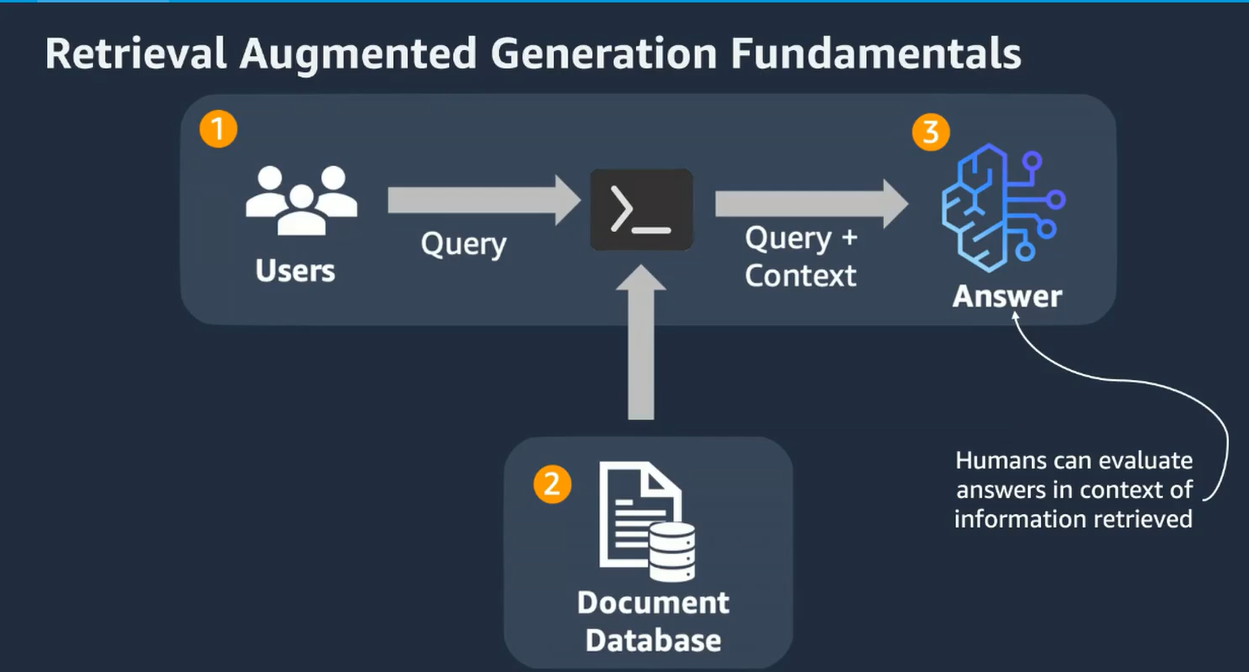
\includegraphics[width=0.90\textwidth]{images/Screenshot 2025-04-02 214315.png}
    \caption{Productizing Healthcare ChatBots with John Snow Labs' Medical LLM-as-a-Judge, Healthcare NLP Summit 2025, John Snow Labs. \url{https://app.swapcard.com/event/healthcare-nlp-summit-2025/planning/UGxhbm5pbmdfMjU3Njg5Ng==}}
    \label{fig:RAG}
\end{figure}

\subsubsection{RAG Pipeline}
A RAG pipeline retrieves patient note chunks that are relevant to the input query, and then appends them to the query. The retriever uses an encoder model to represent both the query and contextual information in the embedding space, and its goal is to retrieve the specific information whose embeddings are close to that of the query. A challenge in RAG-based methods is to ensure that the retrieved information is relevant to the query, and does not contain information that will disrupt LLM reasoning and/or delay inference \cite{clinicalentityIE2025}. The same great challenge was present in the initial stages of this project, as it was very difficult to retrieve chunks of a certain patient. What used to happen was that retrieved chunks used to involve various patients, most probably because all of the patient files had very similar information structure. The problem was solved by experimenting with the chunk content as seen below.

\subsubsection{Mock Data / Data Curation}
For the retrieval part, a database of clinical notes was required. In this project, actual, proprietary data from a real-world clinic were not made available due to privacy concerns, this is why mock data were used. The fifty clinical notes that were created were based on the three interviews, e.g. regarding the structure (lists), the topics covered (basic information, diagnoses, treatment, etc.), the language (note-taking style). In addition, some patient notes were enriched with a different structure (free-form text) and more or fewer topics, in order to represent other forms of patient notes as well. The first ten were created manually with great care to mimic actual patient records, while the rest were generated by \textit{ChatGPT} synthetically, and based on the first ten.

All experimentation occurred on Kaggle notebooks with an accelerator of 2 (two) Tesla T4 GPUs of 15 GB each.

\subsection{First experiment with LLM: Gemma\_trained\_for\_Greek}
I first started experimenting with “Gemma\_trained\_for\_Greek” of 2 B parameters, which I downloaded from Kaggle \footnote{Gemma\_trained\_for\_Greek, Accessed May 2025. \url{https://www.kaggle.com/models/soloupis/gemma\_trained\_for\_greek}}, the sentence transformer embedding model "sentence-transformers/paraphrase-multilingual-MiniLM-L12-v2", as it is multilingual and includes Greek, and the FAISS vector database. 

To add a memory component during inference, I used two custom functions: one to extract the current patient’s name from the query, and the second to resolve personal pronouns such as \textgreek{του, της, αυτήν}, etc. and replace the pronoun with the latest patient’s name. Only later did I learn the LangChain had a built-in memory module, so I used it in my next experiment (see Section \ref{krikri}).

The constraints of this approach were not unimportant: first, the query had to have a pronoun in order for the custom memory to work, and second, the system crashed after 3 queries due to the available Kaggle GPU (VRAM) memory threshold of 30 GB. I experimented with one (1), and then with two (2) patients. As it is obvious from the examples below, the results with one patient were mostly fine, but with two patients they were disappointing, as the answers were either incorrect or mixed-up, or contained English words.

\subsubsection{One patient (MARIA.txt)}

Experimental Query 1: \textgreek{Η Μαρία Παπαδοπούλου τι αγωγή παίρνει στην παρούσα φάση?} \\
System - golden: \textgreek{Η Μαρία Παπαδοπούλου παίρνει αλπραζολάμη για τις κρίσεις πανικού με δοσολογία 0,5 mg και πρόγραμμα 2 φορές την ημέρα.} \\
System - actual: \textgreek{Η Μαρία Παπαδοπούλου παίρνει αλπραζολάμη με δοσολογία (0.5 m}g) \textgreek{και πρόγραμμα 2 φορές την ημέρα.} \\
\\
Experimental Query 2: \textgreek{Και σε ποια δραστική ουσία έχει παρενέργειες αυτή?} \\
Resolved Query 2: \textgreek{Και σε ποια δραστική ουσία έχει παρενέργειες Μαρία Παπαδοπούλου?}
System - golden: \textgreek{Στο λίθιο.} \\
System - actual: \textgreek{Η Μαρία Παπαδοπούλου έχει παρενέργειες από το λίθιο.}\\
\\
Experimental Query 3: \textgreek{Πότε είναι οι επόμενες αιματολογικές της εξετάσεις?} \\
Resolved Query 3: \textgreek{Πότε είναι οι επόμενες αιματολογικές Μαρία Παπαδοπούλου εξετάσεις?} \\
System - golden: \textgreek{Στις 15 Μαΐου 2025.} \\
System - actual: \textgreek{Οι επόμενες αιματολογικές εξετάσεις της Μαρίας Παπαδοπούλου είναι στις 15 Μαΐου 2025.}\\
\\
Experimental Query 4: \textgreek{Πες μου την αγωγή του Κώστα Καρά.} \\
Resolved Query 4: \textgreek{Πες μου Κώστα Καρά αγωγή Κώστα Καρά Κώστα Καρά.} \\
System - golden: \textgreek{Παίρνει σερτραλίνη των 50} mg, 1 \textgreek{φορά το πρωί και ραμιπρίλη των 5} mg 1 \textgreek{φορά το πρωί.} \\
System - actual: \textgreek{Δεν έχω αρκετές πληροφορίες για να απαντήσω στην ερώτηση.Θα μπορούσατε να παρέχετε περισσότερα πλαίσια ή πληροφορίες για να μπορέσω να απαντήσω στην ερώτηση?}\\

\subsubsection{Two patients (MARIA.txt, KOSTAS.txt)}

Experimental Query 1: \textgreek{Η Μαρία Παπαδοπούλου τι αγωγή παίρνει στην παρούσα φάση?} \\
System - golden: \textgreek{Η Μαρία Παπαδοπούλου παίρνει αλπραζολάμη για τις κρίσεις πανικού με δοσολογία 0,5 mg και πρόγραμμα 2 φορές την ημέρα.} \\
System - actual: \textgreek{Δεδομένων των απαντημένων πληροφοριών, δεν είναι γνωστό ποια φάρμακα παίρνει η Μαρία Παπαδοπούλου. Θα μπορούσατε να παρέχετε περισσότερα στοιχεία ή πληροφορίες για να μπορέσετε να απαντήσετε στην ερώτηση?} \\
\\
Experimental Query 2: \textgreek{Και σε ποια δραστική ουσία έχει παρενέργειες αυτή?} \\
Resolved Query 2: \textgreek{Και σε ποια δραστική ουσία έχει παρενέργειες Μαρία Παπαδοπούλου?}
System - golden: \textgreek{Στο λίθιο.} \\
System - actual: \textgreek{Η Μαρία Παπαδοπούλου έχει παρενέργειες από τη δραστική ουσία ολανζαπίνη.}\\
\\
Experimental Query 3: \textgreek{Πότε είναι οι επόμενες αιματολογικές της εξετάσεις?} \\
Resolved Query 3: \textgreek{Πότε είναι οι επόμενες αιματολογικές Μαρία Παπαδοπούλου εξετάσεις?} \\
System - golden: \textgreek{Στις 15 Μαΐου 2025.} \\
System - actual: \textgreek{Οι επόμενες αιματολογικές εξετάσεις της Μαρίας Παπαδοπούλου είναι} scheduled \textgreek{για την 15/5/2025}\\
\\
Experimental Query 4: \textgreek{Πες μου την αγωγή του Κώστα Καρά.} \\
Resolved Query 4: \textgreek{Πες μου Κώστα Καρά αγωγή Κώστα Καρά Κώστα Καρά.} \\
System - golden: \textgreek{Παίρνει σερτραλίνη των 50} mg, 1 \textgreek{φορά το πρωί και ραμιπρίλη των 5} mg 1 \textgreek{φορά το πρωί.} \\
System - actual: \textgreek{Δεν υπάρχουν αρκετές πληροφορίες για να καθοριστεί η αγωγή για τον Κώστα Καρά. Θα μπορούσατε να παρέχετε περισσότερα δεδομένα ή συγκεκριμένες παραγγελίες για να μπορέσετε να καθορίσετε την αγωγή του Κώστα Καρά?}\\


\subsection{Second experiment with LLM: KriKri} \label{krikri}
Then, I experimented with the quantized version of the LLM "ilsp/Llama-Krikri-8B-Instruct", because it was one of the newest models at that time (in May 2025) promising advanced language capabilities in both Greek and English - my two languages of interest - and an expanded context window of 128k tokens \footnote{Llama-Krikri-8B, 9 Feb 2025, \url{https://www.ilsp.gr/en/news/krikri/}} . For this instruction-focused LLM I added the following custom template to minimize hallucinations: \textgreek{Είσαι το Κρικρί, ένα εξειδικευμένο μοντέλο Τεχνητής Νοημοσύνης για ιατρικά δεδομένα. Απάντησε μόνο με βάση τα έγγραφα και την ιατρική πληροφόρηση που έχεις πρόσβαση. Αν δεν ξέρεις την απάντηση, πες ότι δεν ξέρεις.}. Αs an improvement from the previous custom memory, I added LangChain’s ``ConversationBufferMemory``. I also used LangChain’s``ConversationalRetrievalChain`` to connect the memory to the LLM’s prompt as ``chat history`` together with the query and the context from the FAISS database. Despite the memory boost, due to the available Kaggle GPU (VRAM) memory threshold of 30 GB, the system was still crashing after the third query, as the LLM model occupied almost half of the available memory (16 GB). I started experimenting with 2 patients reaching up to 8 patients, past which the results deteriorated, and the answers were mixed-up or plainly wrong, e.g.:

\subsubsection{Eight patients}

Experimental Query 1: \textgreek{Η Μαρία Παπαδοπούλου τι αγωγή παίρνει στην παρούσα φάση?} \\
System - golden: \textgreek{Η Μαρία Παπαδοπούλου παίρνει αλπραζολάμη για τις κρίσεις πανικού με δοσολογία 0,5 mg και πρόγραμμα 2 φορές την ημέρα.} \\
System - actual: \textgreek{Η πληροφορία που παρέχεται δεν περιέχει δεδομένα για ασθενή με όνομα Μαρία Παπαδοπούλου. Οι περιπτώσεις αφορούν τις ασθενείς Γεωργία Αναστασιάδη, Γεωργία Μαντά και Κώστα Καρά.} \\
\\
Resolved Query 2: \textgreek{Και σε ποια δραστική ουσία έχει παρενέργειες Μαρία Παπαδοπούλου?}
System - golden: \textgreek{Στο λίθιο.} \\
System - actual: \textgreek{Η δραστική ουσία που προκαλεί παρενέργειες στην παρούσα φάση για τη Γεωργία Αναστασιάδη είναι η βουπροπιόνη, με αναφερόμενες παρενέργειες την ταχυκαρδία και την αϋπνία.}\\
\\
Experimental Query 3: \textgreek{Πότε είναι οι επόμενες αιματολογικές της εξετάσεις?} \\
System - golden: \textgreek{Στις 15 Μαΐου 2025.} \\
System - actual: \textgreek{Δεν υπάρχουν πληροφορίες για ασθενή με όνομα Μαρία Παπαδοπούλου στο παρεχόμενο ιατρικό ιστορικό.}\\
\\
Experimental Query 4: \textgreek{Πες μου την αγωγή του Κώστα Καρά.} \\
System - golden: \textgreek{Παίρνει σερτραλίνη των 50} mg, 1 \textgreek{φορά το πρωί και ραμιπρίλη των 5} mg 1 \textgreek{φορά το πρωί.} \\
System - actual: \textgreek{Δεν υπάρχουν πληροφορίες για ασθενή με όνομα Κώστας Καρά στο παρεχόμενο ιατρικό ιστορικό.}\\


\section{Technical implementation of the Baseline system}
After experimenting with the two LLMs described above, I moved on to a less memory-intensive solution using Gemini Flash via an API call, as it allowed for more sequential queries. This evolved into my baseline system.

\subsection{Chunking}
In the baseline system, each patient’s text file was first loaded and annotated with the patient’s name as metadata. To enable efficient retrieval, the documents were then segmented into smaller, overlapping chunks using the ``Recursive Character Text Splitter``. This splitter was chosen as it maintains semantic coherence while respecting character boundaries and hierarchical structures (i.e. first sentences, then paragraphs, and then words) within a document \footnote{"How to Use RecursiveCharacterTextSplitter in LangChain". Gary Svenson. Medium (blog), Last accessed July 6, 2025.  \url{https://medium.com/towards-agi/how-to-use-recursivecharactertextsplitter-in-langchain-23bcb0448fca}}. Each chunk was limited to 800 characters with an overlap of 100 characters, ensuring continuity of context between adjacent segments while avoiding excessive fragmentation. 

\subsection{Embedding Model}
The chunks were then converted into numerical representations. The embedding model that was used was the multilingual ``sentence-transformers/paraphrase-multilingual-MiniLM-L12-v2`` because Greek language was included in its training data and because of its suitability in semantic search \footnote{HuggingFace, ModelCard for sentence-transformers/paraphrase-multilingual-MiniLM-L12-v2, Accessed July 5, 2025. \url{https://huggingface.co/sentence-transformers/paraphrase-multilingual-MiniLM-L12-v2}}. 

\subsection{Vectorstore}
The resulting embeddings of the chunks, enriched with metadata, were later stored in a \textit{Faiss} vector index for similarity-based retrieval. For retrieval, the system was configured with k = 3, meaning that the three most semantically similar chunks were returned for each query. This relatively small value of k was chosen to reduce noise and ensure that only the most relevant context was passed to the LLM, thereby improving answer precision.

\subsection{LLM}
The baseline system was based on Google's LLM ``gemini-2.0-flash`` model, which was integrated through the \textit{LangChain} framework. This model was chosen because of its very good performance and instruction-following capability, support of the Greek language, and generally better results than other Gemini models, even ``gemini-2.5-flash`` \footnote{Google Cloud (blog). Gemini 2.0 Flash. Accessed on July 5, 2025. \url{https://cloud.google.com/vertex-ai/generative-ai/docs/models/gemini/2-0-flash}}. The model was configured with a low temperature (set to 0.2) for consistent and deterministic responses, which is especially important in the clinical domain. A customized system prompt written in Greek defined the model's behavior: \textgreek{Είσαι ένας πρόθυμος και φιλικός βοηθός νοσηλευτών σε ελληνική ψυχιατρική κλινική. Πρέπει να απαντάς σε κάθε ερώτηση. Οι ερωτήσεις αφορούν συγκεκριμένα ιατρικά και προσωπικά δεδομένα ή περιλήψεις όλων των δεδομένων ενός ασθενή. Οι ερωτήσεις και τα ονόματα των ασθενών είναι στα ελληνικά. Χρησιμοποίησε τόσο την ερώτηση όσο και το ιστορικό συνομιλίας όταν αποφασίζεις ποιο εργαλείο να καλέσεις ή πώς να απαντήσεις. Αν δεν είσαι σίγουρος για το όνομα του ασθενούς ή αν έχεις δύο ασθενείς με το ίδιο όνομα, ρώτα για ποιον να ψάξεις. Πρέπει να είσαι σίγουρος ότι η απάντηση που δίνεις αφορά τον ασθενή της ερώτησης. Απάντα στα ελληνικά και αποκλειστικά με βάση τα παρεχόμενα δεδομένα. Αν δεν βρίσκεις την απάντηση στα δεδομένα, πες ότι δεν υπάρχει.}. In addition, a structured RAG prompt template was added to inject the necessary context into each query. This template incorporated the conversation history, the retrieved document chunks, and the user’s query, ensuring that the model grounded its responses in the available patient data rather than hallucinating unsupported information.

\subsection{Memory}
To support conversational continuity, the system employed ``ConversationBufferWindowMemory`` from \textit{LangChain}. This component maintained a history of the most recent dialogue turns, storing both user inputs and model outputs. The window size was set to 3, as the expected interactions by the nurses are supposed to be brief and straightforward. In this way, the memory preserved the three latest conversations without overwhelming the LLM model with the entire dialogue history. This enabled the system to correctly interpret follow-up questions, resolve references to previous queries, and sustain natural multi-turn interactions.

\subsection{Chain}
The language model, the retriever, the custom prompt, and the memory component were integrated into a ``ConversationalRetrievalChain``. At each query, the chain retrieved the most relevant document chunks from the vector store, combined them with the current conversation history stored in memory, and passed them into the custom RAG prompt template. The Gemini 2.0 Flash model, then, generated a response conditioned on both the retrieved knowledge and the conversational flow. The chain was further configured to return the source documents used in each response, ensuring transparency and enabling later evaluation of grounding accuracy.

\section{Technical implementation of System 1}

In addition to the RAG/LLM setup, I added two helpful functions (tools) and an reasoning agent. I used the \textit{LangChain} open-source framework to connect the four components (data source, LLM, tool calling, and agent) into a chatbot application. All components will be analyzed below.

\subsection{Chunking}
The data documents were split based on 550-character chunks with a 50-character overlap via the ``RecursiveCharacterTextSplitter``. Since all patient data contain similar information, it was originally difficult for the retriever to pinpoint the chunk for the correct patient, as mentioned above. The above experimentation showed that prefixing each chunk with the patient name and their Social Security Number (AMKA) was ideal for identifying the correct chunk.

Moreover, appending the patient name as metadata created the basis for tool calling at a later stage, which further ensured accurate retrievals.

\subsection{Embedding Model}
The chunks were then converted into numerical representations. The embedding model that was used was the multilingual ``sentence-transformers/paraphrase-multilingual-MiniLM-L12-v2`` as described above. Also, this model was preferred over others in general due to its better performance in semantic similarity scoring compared to others, even Greek Bert models \footnote{HuggingFace, Model Card for nlpaueb/bert-base-greek-uncased-v1 \url{https://huggingface.co/nlpaueb/bert-base-greek-uncased-v1} and Model Card for https://huggingface.co/nlpaueb/legal-bert-base-uncased \url{nlpaueb/legal-bert-base-uncased}, Accessed July 5, 2025.}.

\subsection{Vectorstore}
After gathering the embeddings of all the split chunks, these were put into the vector database \textit{Chroma}. \textit{Chroma} was ultimately selected over \textit{Faiss} because of its native support of metadata. This means that the former can filter by a piece of metadata -- in this project, the patient's name -- during its retrieval, whereas the latter cannot.

\subsection{LLM}
The LLM used was again ``gemini-2.0-flash`` for the reasons described in the Baseline system above, as well as because of its suitability for function (tool) calling, and its use with agents. Especially important was the model's ample context window of 1 million tokens, since the length of patient notes together with the memory (chat history) can easily surpass an LLM’s context window. The model was configured with a very low temperature (set to 0.2) for consistent and deterministic responses, which is especially important in the clinical domain. I kept the same customized system prompt as described in the Baseline system above to define the model's behavior as a friendly assistant for Greek-speaking psychiatric nurses. The prompt ensured the responses are always in Greek, are patient-specific, and grounded strictly in the provided data as well as the chat history. Also, the prompt encouraged tool use and enforced responsible handling of ambiguous queries, such as those involving duplicate patient names.

\subsection{Memory}
To maintain conversational continuity and  help the assistant disambiguate patient references across multiple queries, a memory component was added via ``LangChain's ConversationBufferMemory``. This component preserves the dialogue history throughout the interaction, allowing the agent to reference earlier parts of the conversation when formulating responses. This functionality is particularly important in a clinical environment where users often ask follow-up questions based on earlier responses.

\subsection{Tools} \label{tools}
To enhance the agent's reasoning capabilities and modularity, the system incorporated a tool-based architecture using LangChain’s ``@tool`` decorator. Tools are basically callable functions that the language model can invoke when specific types of reasoning or external data access is required. Two custom tools were implemented: one to extract the patient name, and the other to get the relevant patient documents. 
The first tool is responsible for identifying the patient’s full name in Greek, either directly from the current user query or from the conversation history. This disambiguation step is critical for keeping document retrieval patient-specific, especially when users omit or reference names indirectly (e.g. by using personal pronouns). 
The second tool, performs a filtered retrieval from the \textit{Chroma} vector store using the patient's name as a metadata piece, returning only relevant chunks. This filtered retrieval ensures that only pertinent information is passed to the LLM.

\subsection{Agent}
Recently, AI agents (or ``agentic AI``) have become more and more popular, with a focus on logistics support, and assistive roles in long-term care \footnote{``AI Use-Case Compass — Healthcare: Intelligent Care, Delivered``, Adnan Masood, PhD., Medium (blog), Accessed June 28, 2025. \url{https://medium.com/@adnanmasood/ai-use-case-compass-healthcare-intelligent-care-delivered-ab27d8f8f610}}. Agents can achieve specific goals autonomously, by interpreting information, making decisions, and taking actions without needing step-by-step human instruction, but by leveraging certain tools at its disposal (see Section \ref{tools}). They are designed to handle more complex problems that require planning, adaptation, and coordination across different types of data and tasks \footnote{``The age of AI agents - Reasoning, autonomy, workflows, and LEGO blocks?``, Dr Josh Au Yeung, LinkedIn (blog), Accessed July 10, 2025. \url{https://www.linkedin.com/pulse/age-ai-agents-reasoning-autonomy-workflows-lego-blocks-au-yeung-qm3ke/}}.

The dialog management was managed by a \textit{LangChain} agent, which served as the orchestrator among the language model, the tools, and the memory. The agent was initialized using an architecture that was designed to enable the model to reason step-by-step about which tool to invoke based on the conversation. This agent type (``AgentType.STRUCTURED\_CHAT\_ZERO\_SHOT\_REACT\_DESCRIPTION``) is particularly effective in scenarios that require interpretable decision-making, as it encourages the model to ``think aloud`` and choose actions in a structured manner. The agent was configured with access to custom tools and long-term memory, allowing it to retrieve patient-specific data and handle follow-up questions spanning multiple conversational turns. The extra parameter ``handle\_parsing\_errors=True`` ensured well formatted LLM outputs, while ``return\_intermediate\_steps=True`` allowed access to the retrieved documents and also helped in debugging of the reasoning process.

\section{Technical implementation of System 2}
To improve the naturalness of the system’s answers I did some LLM hyperparameter tuning and edited the prompt slightly adding the sentence \textgreek{"Να απαντάς με φυσικό και καθησυχαστικό τόνο, σαν να μιλάς σε συνάδελφο."}. To improve the scores from RAGAS evaluation, I made some changes as well. System 2 is identical to System 1 except for the LLM tuning, and the text to speech component.

Regarding hyperparamter tuning, I tried to make the dialog more natural, but still safe and accurate. Temperature was raised to 0.6 from 0.2 in System 1 for reducing the ``robotic`` feel, and for adding a bit of variability and ``naturalness`` in the responses, but still avoiding hallucinations. Then, top\_p was set to 0.9 in comparison to the default 1 value of System 1 for a little more coherent text and less diverse (fewer rare words) wording \footnote{`How to generate text: using different decoding methods for language generation with Transformers`. Edited July 2023. Accessed on September 14 2025. \url{https://huggingface.co/blog/how-to-generate}}. Moreover, I added the following instruction to the prompt: ``\textgreek{Να απαντάς με φυσικό και καθησυχαστικό τόνο, σαν να μιλάς σε συνάδελφο.}`` to enhance text naturalness.

Regarding the speech component, I decided ton Coqui's TTS, as the best choice among the rest few free-of-charge TTS systems for Greek (e.g. Meta's MMS-TTS Greek model \footnote{facebook/mms-tts-ell. \url{"facebook/mms-tts-ell"}}). The Greek model `tts\_models/el/cv/vits` was selected, in combination with a dates normalization and miligram function for a more natural Greek pronunciation.

\section{Evaluation}
Evaluation is essential to verify the benefits and effectiveness of this question-answering assistant. Evaluating LLMs presents certain challenges due to their generative nature and lack of precise ground truth data. Traditional evaluation metrics used for discriminative models are often insufficient for assessing the quality, coherence, diversity, and usefulness of LLM-generated text. Below are the traditional evaluation metrics: WER (how many insertions, deletions, and substitutions required to transform the candidate into the reference string), Exact Match (measures accuracy), BLEU (how many n-grams in the generated text appear in the reference text), ROUGE (measures recall). Other metrics relevant to LLMs include precision (correctness), recall (completeness, i.e. reliability) of patient progress notes, and inference time (latency). However, these cannot evaluate semantics and context, as they are only focusing on word counts. Evaluating RAG systems is not straightforward either. As explained by \citeauthor{ragas2025} (2025), the RAGAs framework inventors, ``While the usefulness of retrieval-augmented strategies is clear, their implementation requires a significant amount of tuning, as the overall performance will be affected by the retrieval model, the considered corpus, the LM, or the prompt formulation, among others.`` It becomes obvious that all the above factors need to be measured and evaluated.

\subsubsection{Quantitative Analysis}
The RAGAs (Retrieval-Augmented Generation Assessment) framework is very popular for evaluating RAG applications. RAGAs uses LLMs under the hood to conduct the evaluation under various metrics. 
The metrics that were used in this project were the following \footnote{rag-langchain-ragas (git repository), Accessed July 8, 2025.\url{https://github.com/benitomartin/rag-langchain-ragas}}:

\begin{enumerate}
\item Faithfulness (context Vs answer) \footnote{Ragas (website). Accessed July 1, 2025. \url{https://docs.ragas.io/en/latest/howtos/integrations/langchain/##evaluate}}: It measures generated hallucinations by assessing whether all claims in the generated answer can be inferred directly from the provided context. It is calculated from the answer and the retrieved context. The answer is scaled to a (0,1) range, and the higher score is the better. It answers to the question: ``Is the generated answer grounded to the context? ``
\item Answer Relevancy (question Vs answer): It evaluates answer quality by assessing how relevant the generated answer is to the question. A lower score is assigned to answers that are incomplete or contain redundant information. This metric is computed using the question and the answer, with values ranging between 0 and 1, where higher scores indicate better relevancy. It answers to the question: ``Is the generated answer appropriate to the question? ``
\item Answer Correctness (ground truth Vs answer): Assesses the accuracy of the generated answer when compared to the ground truth. This evaluation relies on the ground truth and the answer, with scores ranging from 0 to 1. A higher score indicates a closer alignment between the generated answer and the ground truth, signifying better correctness. It answers to the question: ``How close is the generated answer to the ground truth? ``
\item Context Precision (retrieved context Vs question): It checks if the retriever gave relevant, i.e. non-redundant, content by assessing whether all golden chunks that are present in the retrieved contexts are ranked high, as they should ideally. This metric is computed using the question and the contexts, with values ranging between 0 and 1, with higher scores indicating better precision. It answers to the question: ``How useful the retrieved context is to answering the question? ``
\item Context Recall (retrieved context Vs ground truth): It checks if all golden facts were present by measuring the extent to which the retrieved context aligns with the golden answer. It is computed based on the ground truth and the retrieved context, and the values range between 0 and 1, with higher values indicating better performance. It answers to the question: ``Did the retriever retrieve all the golden chunks? ``
\end{enumerate}

\section{Discussion} 
This study utilized a variety of simulated patients for the specialty of psychiatry. For its evaluation both quantitative and qualitative methods were used. First, the evaluation results from the RAGAs frameowrk will be presented, and second the results from the questionnaire.

\subsection{Results from RAGAs framework for Baseline}
\subsection*{Summary Table - Average Metrics}
The following table provides a high-level summary of how well the Baseline system performs in general.

\begin{table}[ht]
\centering
\begin{tabular}{l c}
\toprule
\textbf{Evaluation Metric} & \textbf{Average Score} \\
\midrule
Faithfulness          & 0.802 \\
Answer Relevancy      & 0.347 \\
Answer Correctness    & 0.316 \\
Context Precision     & 0.548 \\
Context Recall        & 0.399 \\
\bottomrule
\end{tabular}
\caption{Baseline - Average scores for RAGAs metrics}
\label{tab:ragas_avg_metrics_baseline}
\end{table}

\subsection*{Summary Plot}
The following is a bar plot that compares the average score for each metric across the 25 queries.

\begin{figure}[H]
  \centering
  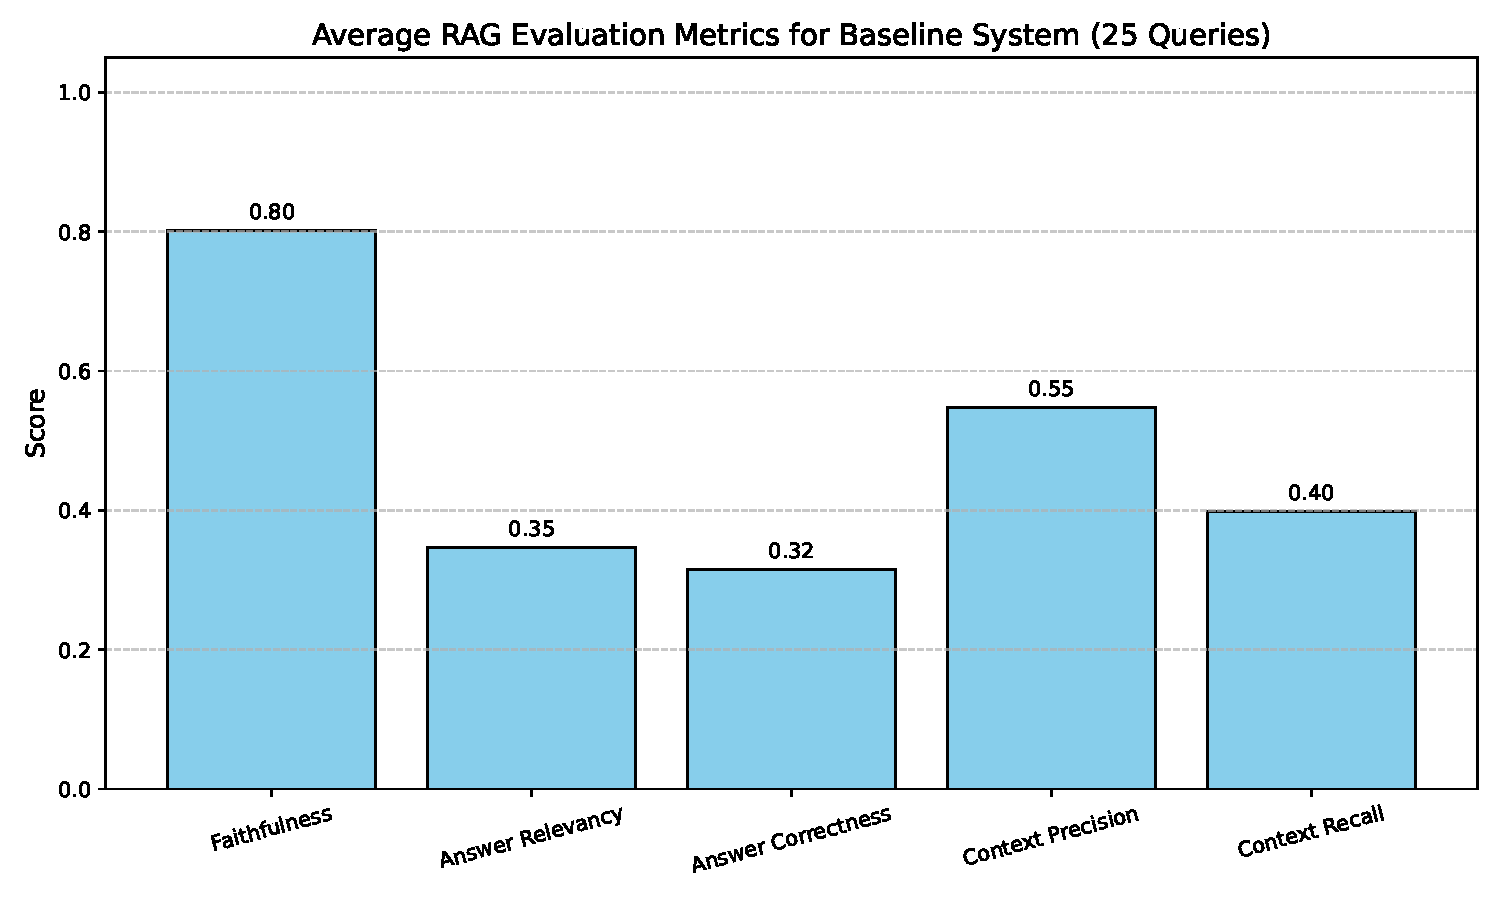
\includegraphics[width=1\textwidth]{Chapter2/ragas_avg_plot-baseline.pdf}
  \caption{Average scores for RAGAs metrics across 25 queries}
  \label{fig:ragas_avg_metrics} 
\end{figure}

The metric of \textit{faithfulness} showed a high average score (0.802), indicating that the model’s responses were very close to the retrieved content, without hallucinations of extra facts.

The metric of \textit{answer relevancy} is quite low (0.35), which indicates that many answers are not directly aligned with the user query. The reason may be that the retriever returned chunks that are related but not very specific, hence the generated answers were incomplete or contain redundant information.

\textit{Answer correctness} has the lowest score (0.32), meaning that the actual information in the responses does not match the ground truth. This indicates that either the context coming from the retriever is not the right one or that the LLM does not choose the right facts from the retrieved chunks to generate its answer.

\textit{Context precision} is almost random at 0.55, indicating that only about half of the retrieved context is really relevant to the query. This means that the other half is redundant information, which can explain the low scores for \textit{answer relevancy} and \textit{answer correctness} described above.

Finally, the metric of \textit{context recall} is quite low (0.39), indicating that the retriever frequently fails to capture all of the necessary context. This score, like the score for \textit{context precision},  can also explain low \textit{answer relevancy} and \textit{answer correctness}.

The overall picture is that the baseline system is faithful (0.80), i.e. it does not hallucinate much, which shows that the system prompt and LLM choice manage to constrain the model to retrieved context. The problem, though, lies in the retrieval quality, because the retriever mostly misses relevant passages (context recall = 0.39) and adds irrelevant information (context precision = 0.55). This is why for System 1 I focused in improving the chunking process, changed the vector database from \textit{Faiss} to \textit{Chroma}, and added the tools and the agent.


\subsection{Results from RAGAs framework for System 1}
\subsection*{Summary Table - Average Metrics}
The following table provides a high-level summary of how well System 1 performs in general.

\begin{table}[ht]
\centering
\begin{tabular}{l c}
\toprule
\textbf{Evaluation Metric} & \textbf{Average Score} \\
\midrule
Faithfulness          & 0.739 \\
Answer Relevancy      & 0.520 \\
Answer Correctness    & 0.634 \\
Context Precision     & 0.740 \\
Context Recall        & 0.781 \\
\bottomrule
\end{tabular}
\caption{System 1 - Average scores for RAGAs metrics}
\label{tab:ragas_avg_metrics_system1}
\end{table}

\subsection*{Summary Plot}
The following is a bar plot that compares the average score for each metric across the 25 queries.

\begin{figure}[H]
  \centering
  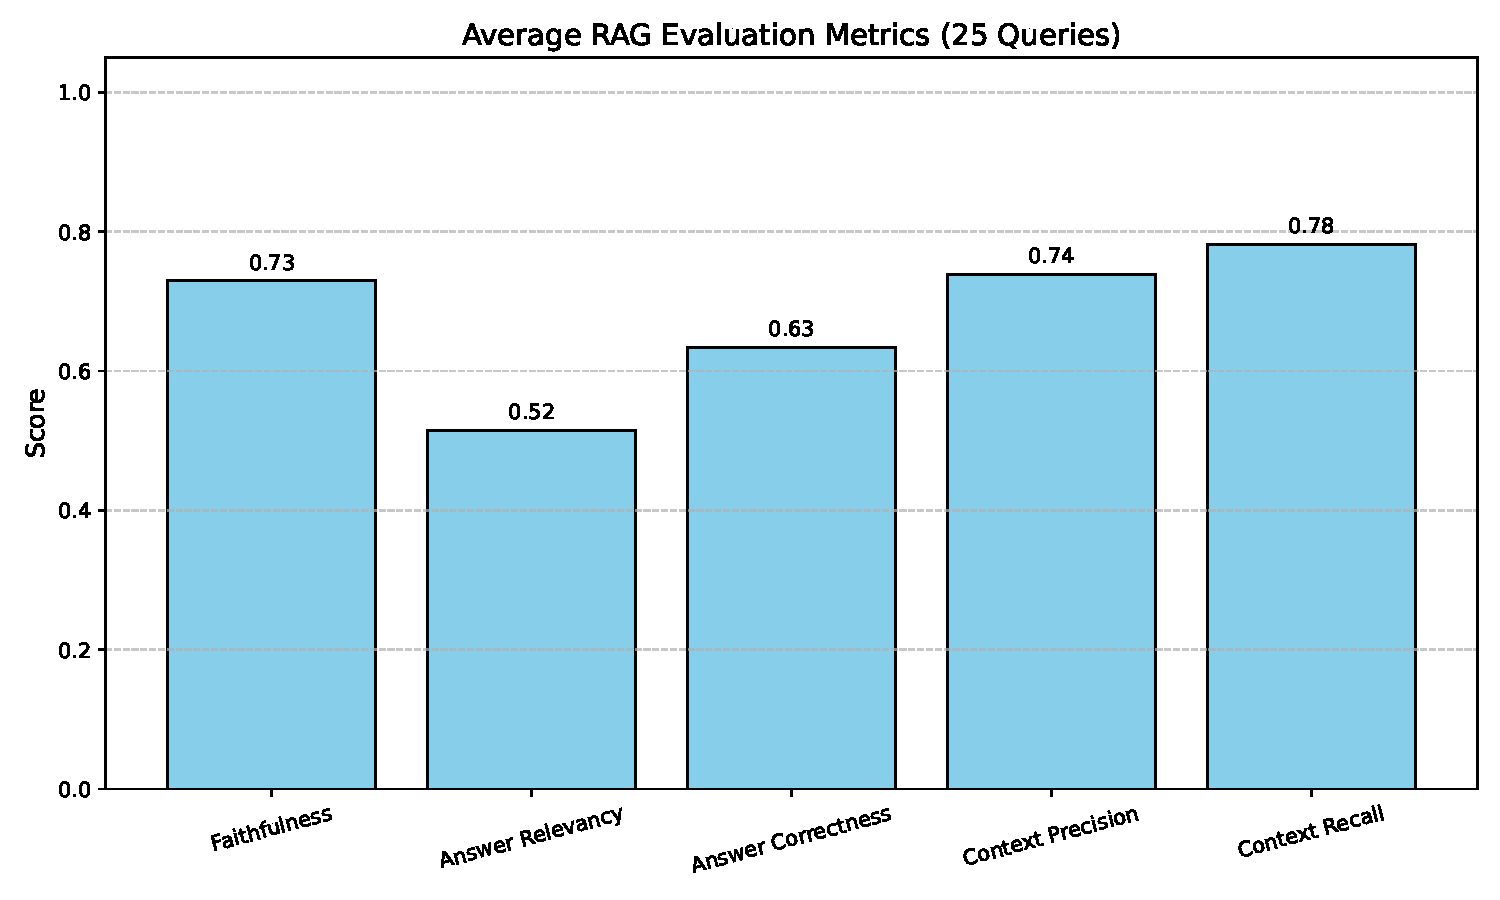
\includegraphics[width=1\textwidth]{Chapter2/ragas_avg_plot-1.pdf}
  \caption{System 1: Average scores for RAGAs metrics across 25 queries}
  \label{fig:sys1_ragas_avg_metrics} 
\end{figure}

The metric of \textit{faithfulness} showed a relatively high average score (0.739), indicating that the model’s responses were generally consistent with the retrieved content.

\textit{Context recall} (0.781) and \textit{context precision} (0.740) were aslo both relatively high, showing that the retrieval component of the assistant effectively selected relevant passages, and that the LLM component has used them efficiently when generating responses. 

\textit{Answer correctness} scored 0.634, showing that there still is room for improvement for the LLM model to produce accurate answers consistently. This low score may be attributed to the fact that the golden answers were in some cases more or less detailed than the generated response, even though both were correct. Notably, \textit{answer relevancy} was the lowest among the metrics (0.520), which implies that while answers were often correct and grounded to the patient data, they did not always fully address the user’s intent or align closely with the query focus.

Overall, the system shows a solid performance in faithfulness and context handling, but would benefit from further enhancements in answer generation.

\subsection*{Individual Plot}
The assistant struggled with the disambiguation of patients with the same name. Specifically, for query nr. 17 (``\textgreek{Δε θυμάμαι το ΑΜΚΑ της. Πες μου για την πιο μικρή.}``) the generated response was ``\textgreek{Δυστυχώς, δεν έχω πληροφορίες για την ηλικία των ασθενών για να προσδιορίσω ποια είναι η πιο μικρή. Παρακαλώ, διευκρινίστε για ποια Δήμητρα Μακρή ενδιαφέρεστε αναφέροντας το ΑΜΚΑ της: 44350232398 ή 41661927592.}``, whereas the golden response is actually the date of the youngest Dimitra Makri's latest hospitalization and her current treatment. The assistant could have retrieved the ages of both patients from the patient data and could have continued the conversation, but failed to do so. This is why almost all the RAGAs metrics for this query equal zero.

\begin{figure}[ht]
    \centering
    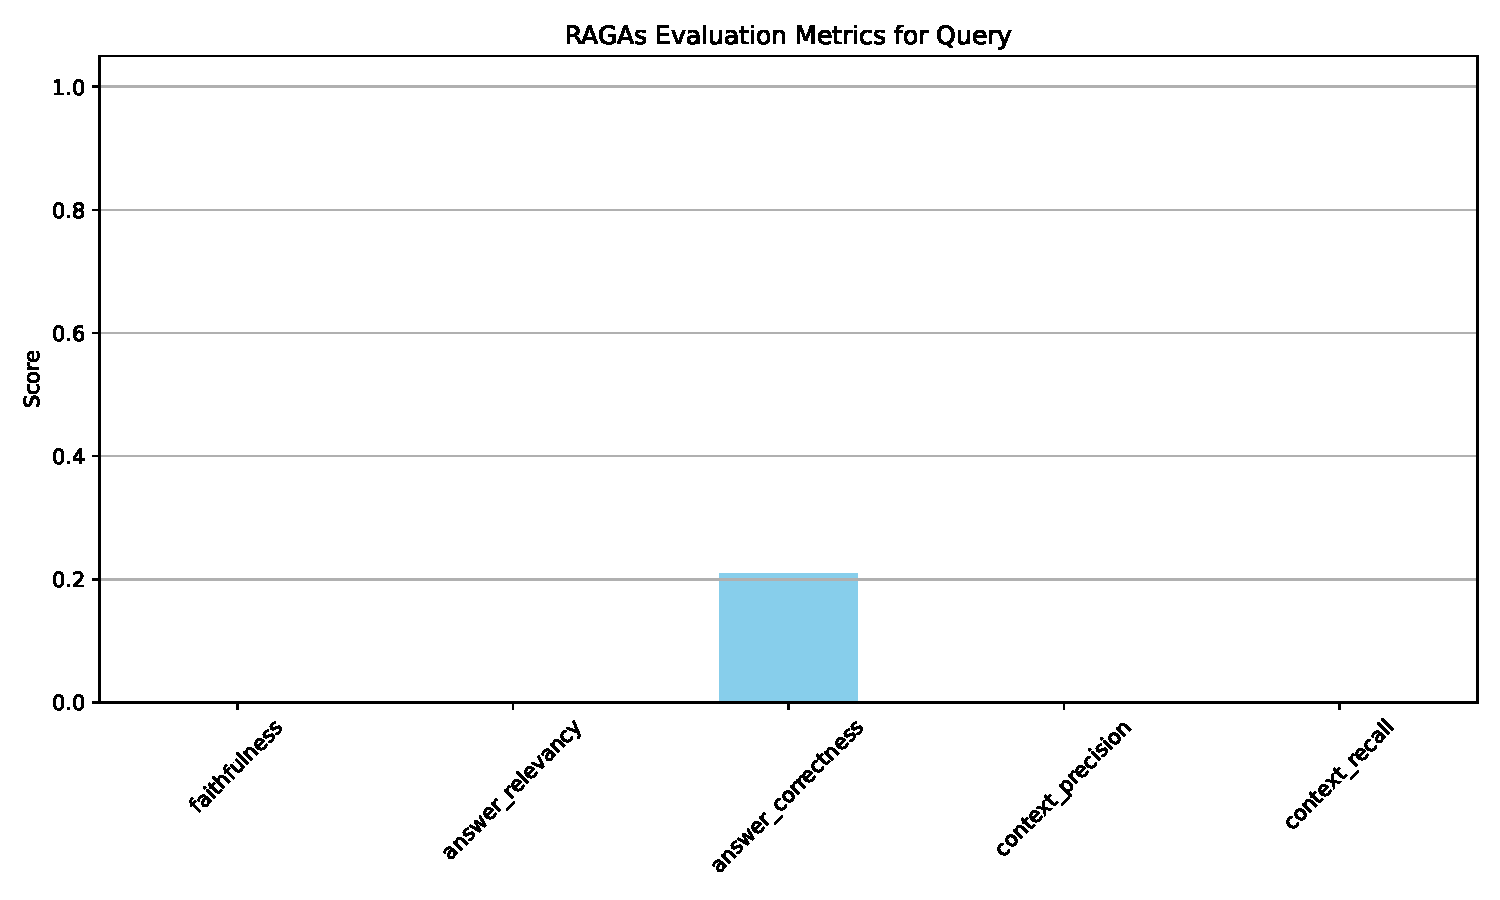
\includegraphics[width=1\textwidth]{Chapter2/metrics_plot_17.pdf}
    \caption{Plot for query nr. 17}
    \label{fig:sys1_ragas_17_metrics}
\end{figure}


\subsection{Results from RAGAs framework for System 2}
\subsection*{Summary Table - Average Metrics}
The following table provides a high-level summary of how well System 1 performs in general.

\begin{table}[ht]
\centering
\begin{tabular}{l c}
\toprule
\textbf{Evaluation Metric} & \textbf{Average Score} \\
\midrule
Faithfulness          & 0.768 \\
Answer Relevancy      & 0.690 \\
Answer Correctness    & 0.700 \\
Context Precision     & 0.840 \\
Context Recall        & 0.790 \\
\bottomrule
\end{tabular}
\caption{System 1 - Average scores for RAGAs metrics}
\label{tab:ragas_avg_metrics_system1}
\end{table}


\subsection*{Summary Plot}
The following is a bar plot that compares the average score for each metric across the 25 queries.

\begin{figure}[H]
  \centering
  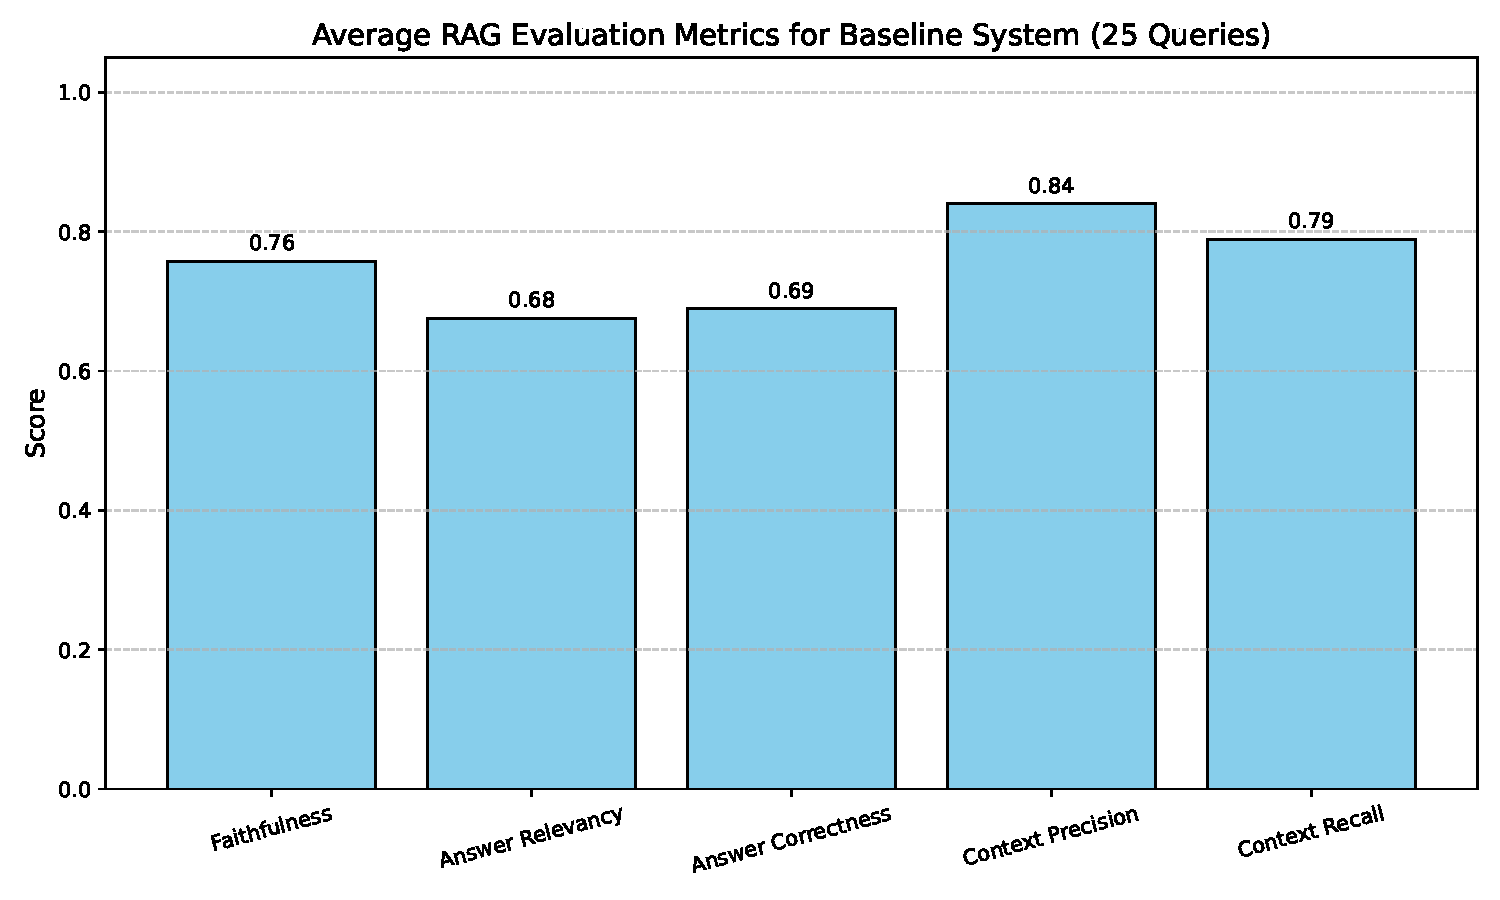
\includegraphics[width=1\textwidth]{Chapter2/SYS2ragas_avg_plot-2.pdf}
  \caption{System 2: Average scores for RAGAs metrics across 25 queries}
  \label{fig:sys2_ragas_avg_metrics} 
\end{figure}

\subsection{Explanation of low scores}
After reviewing the results carefully, it was strikingly apparent that certain test cases had erratic metrics. 

For example, the metric of \textit{faithfulness} was mostly near 1, but in some cases extremely low, or 0 (zero) or even non existent (NaN), because of retrieval gaps in the agent's workflow. The reason is that the agent avoided retrieving the same context twice for follow-up questions of a previous patient name. This resulted in the generated answer being considered as ``unfaithful``.

Linked to retrieval's success or fail are the metrics of \textit{context precision and recall}, whose scores are very high (1) or very low (Nan/0). This extreme scoring exaggerates the gap between partial and complete retrieval failures.

\textit{Answer relevancy} sometimes has NaN value because the LLM judge used by RAGAS judged the answer as failed or as a default (fallback) answer, even though for this case it was not. For example, all answers that correctly state that no information has been found in the retrieved documents or ask for patient disambiguation, got a NaN or a zero value.

About \textit{answer correctness}, this metric has low values because even though the ground truth is precise (exact date, diagnosis, etc.), the response is somewhat vague, incomplete, or a little different (e.g. missing a date or a diagnosis). For example, the generated answer \textgreek{Δεν βρέθηκαν δεδομένα για την Κωνσταντίνα Λυμπερίου} judged against the reference \textgreek{Δεν υπάρχει αυτή η ασθενής} gets a score of only 0.456 in System 2, because the wording is different. Also, even though all rows have their golden answers, RAGAS sometimes doesn’t assign scores (NaN) when the system output is too indirect for a meaningful comparison.

RAGAS's metrics are, of course, designed to be strict and highlight weaknesses in retrieval and generation, like in the systems described above. The relatively low and inconsistent RAGAS scores are partly explained by retrieval gaps in the two systems, but also partly by the strictness of the metrics themselves. The strictness leads to low and erratic scores, which do not always reflect the practical usefulness of the system in a clinical workplace. The NaN and zero values show that RAGAS sometimes totally refuses to evaluate an answer, rather than give a score for the correct part of it. This shows that RAGAS penalizes clinically useful yet incomplete answers much more harshly than a human evaluator would. It can be argued that RAGAS systematically underestimates the systems' performance in a clinical setting, where partial, or approximate answers can still be informative and useful. In short, while the low metrics highlight areas for technical improvement, they should be interpreted with caution and supplemented with human-centered evaluation to better capture the true effectiveness of the voicebot in clinical practice.

\subsection{Results from Questionnaire}
\subsubsection{Qualitative Analysis}
User feedback is essential to understand how real-world users will react to the assistant, as well as identify shortcomings and areas of improvement. Unfortunately, getting direct user feedback from psychiatric nurses was not possible for this project.

Twenty five question-answer pairs were compiled in the form of a questionnaire, and were sent to ten human evaluators. The evaluators were instructed to rank the answers in regards to naturalness and preference by giving a score from 1 (lower/worse) to 5 (higher/better). Two out of ten evaluators were medical professionals (one GP, one gynecologist). Questionnaire results can be found in Appendix~\ref{sec:qresults} and their analysis can be seen in Table~\ref{tab:preferences}.

\subsubsection{Naturalness}
Both System A and System B received very similar average ratings:

A: $2.34  (\sigma = 0.96)$

B: $2.34  (\sigma = 1.09)$

The mode was 2 for both systems, meaning that the score “2” was the most commonly given naturalness score indicating that overall perceived naturalness was fairly low to moderate.

 Scores spanned the full 1–5 range. Distribution is very wide, with some strong positive ratings (up to 5), but most clustered around the lower end.

There is no clear winner in naturalness, as average scores are nearly the same, implying that participants didn’t strongly perceive one system as more natural in isolation.

\subsubsection{Preference}
When asked to choose between the two systems, System A received the majority of the preference vote. Specifically:

64\% preferred A with 160 votes, with human\_9 preferring A 80\% of the times

36\% preferred B with 90 votes, with human\_4 preferring B 52\% of the times 

\begin{table}[H]
\centering
\begin{tabular}{@{}llrr@{}}
\toprule
\textbf{humanEvaluator} & \textbf{Προτίμηση} & \textbf{Count} & \textbf{Percentage (\%)} \\
\hline
human\_1  & A & 16 & 64.0 \\
          & B &  9 & 36.0 \\
human\_10 & A & 13 & 52.0 \\
          & B & 12 & 48.0 \\
human\_2  & A & 14 & 56.0 \\
          & B & 11 & 44.0 \\
human\_3  & A & 18 & 72.0 \\
          & B &  7 & 28.0 \\
human\_4  & A & 12 & 48.0 \\
          & B & 13 & 52.0 \\
human\_5  & A & 17 & 68.0 \\
          & B &  8 & 32.0 \\
human\_6  & A & 17 & 68.0 \\
          & B &  8 & 32.0 \\
human\_7  & A & 18 & 72.0 \\
          & B &  7 & 28.0 \\
human\_8  & A & 15 & 60.0 \\
          & B & 10 & 40.0 \\
human\_9  & A & 20 & 80.0 \\
          & B &  5 & 20.0 \\
\hline
\textbf{Total} & A & 160 & 64.0 \\
               & B &  60 & 36.0 \\
\bottomrule
\end{tabular}
\caption{Preferences (Προτίμηση) for each human evaluator between System A and System B, reported as counts and percentages.}
\label{tab:preferences}
\end{table}
 
This suggests that although the naturalness ratings were almost identical, participants clearly preferred System A when making an explicit choice.

Preference noticeably stands out compared to the ratings. The preference question ``forced`` a choice, and revealed a bias toward System A, even if its naturalness rating was not higher than System B.

\clearpage